\chapter{Dataset}
\label{capitolo6}
\thispagestyle{empty}
\noindent The abundance of astronomical data provides great opportunities for machine learning. In fact, most of the data is free to use for anybody and labels are almost always available. Solar physics is no exception to that. Many public databases of solar events can be downloaded in textual form and then annotations can be reconstructed from them. However, the reconstruction is not trivial sometimes, since a good understanding of solar coordinate systems is required.\\
In this work 4 datasets have been merged together:
\begin{itemize}
  \item \textbf{Debrecen Photoheliographic Data (DPD) \cite{baranyi2016line}\cite{gyHori2016comparative}}: a catalogue of positions and areas of sunspots from 1974 until present times, compiled by using white-light full-disk observations taken at the Heliophysical Observatory of the Hungarian Academy of Sciences (Debrecen, Hungary) and its Gyula Observing Station as well as at other observatories;
  \item \textbf{Sunspot Index and Long-term Solar Observations (SIDC-SILSO) Dataset \cite{clette2014revisiting}}: a time series of daily total sunspot number derived with the relative sunspot number formula \eqref{relssnum}, provided by the Royal Observatory of Belgium using a network of observers. This dataset will be used for validation and testing purposes only;
  \item \textbf{Virtual Solar Observatory (VSO) \cite{hill2009virtual}}: a tool for investigating the physics of the Sun, by searching and downloading existing databases for terrestrial and space-based observations;
  \item \textbf{US Air Force, Mount Wilson (USAF/MWL) Dataset}: a catalogue that provides a list of sunspot regions and their parameters, observed by the USAF solar observatories and the Mount Wilson observatory. In particular, it is famous for sunspot group classification data.
\end{itemize}
The last solar cycle was selected as a use case for the training and testing of the algorithm. Both ground and space telescope data were added up to form a quite large dataset. One full-disk observation was considered for each day, drawn and reconstructed from the DPD dataset. Space based data ranging from 2011 to 2014 was downloaded with a Python module called SunPy \cite{mumford2015sunpy} that connects to VSO's open APIs, while ground based data from 2011 to 2013 was obtained directly from DPD's FTP access. Due to availability problems, the ground observations for 2014 were missing from the database. Since the images came from different datasets some pre-processing was necessary to unify them. Ground based observations came in the form fits files with variable resolution (from 4096x4096 to 8192x8192), where limb darkening correction had already been applied but the disk was not centered in the the plate. So, first, the center, radius and axial tilt of the Sun were extracted from the header in order for the Sun to be aligned and cropped from the raw image. The coordinates of the sunspots were given in the DPD dataset in heliocentric-radial coordinates. From those, using simple trigonometry, it was easy to calculate the positions in pixel coordinates.
On the other hand, the preprocessing of space based observations needed a bit more work. For each day, sunpost instances were extracted from DPD, and SDO images were searched inside the VSO using date and time of the DPD observation. The temporally nearest image was selected and downloaded. Despite the fact that SDO observations are very frequent, the average delay between the image and the annotated mask was around half an hour on average. This time shift is pretty large, considering that the Sun rotates and the Earth moves on the orbit (SDO can be considered solidal to the Earth in this case). The misalignment was big enough to make it necessary to rotate the positions of the sunspots to create very accurate masks. Luckily, DPD also provides Carrington heliographic latitude and longitude for each sunspot. These coordinates can easily be transformed into the helioprojective system. At this point, the images were loaded as a SunPy Map, a class that contains many useful methods to interact with solar data. One of these functions allows to calculate where an helioprojective coordinate maps to, after a time delta, taking into account the differential solar rotation profile. This works well when the sunspots are big because the magnetic tubes that create them usually have a lot of ``inertia'', and therefore move pretty consistently with the rotation profile. Marginal misalignments still arise when sunspots are very small, because even a modest change in the magnetic perturbation causes erratic movements, making it difficult to predict their location. After these calculations, it was the turn of limb darkening correction. From the center of the disk, circles of increasing radius are created and the pixels that lay on the border of the circle are averaged, creating the limb darkening profile (blue points in Figure~\ref{fig:sldtk}). A polynomial function is fitted on these data points and then, for every pixel, the right correction is applied to straighten the profile.
\begin{figure}[t]
    \centering
    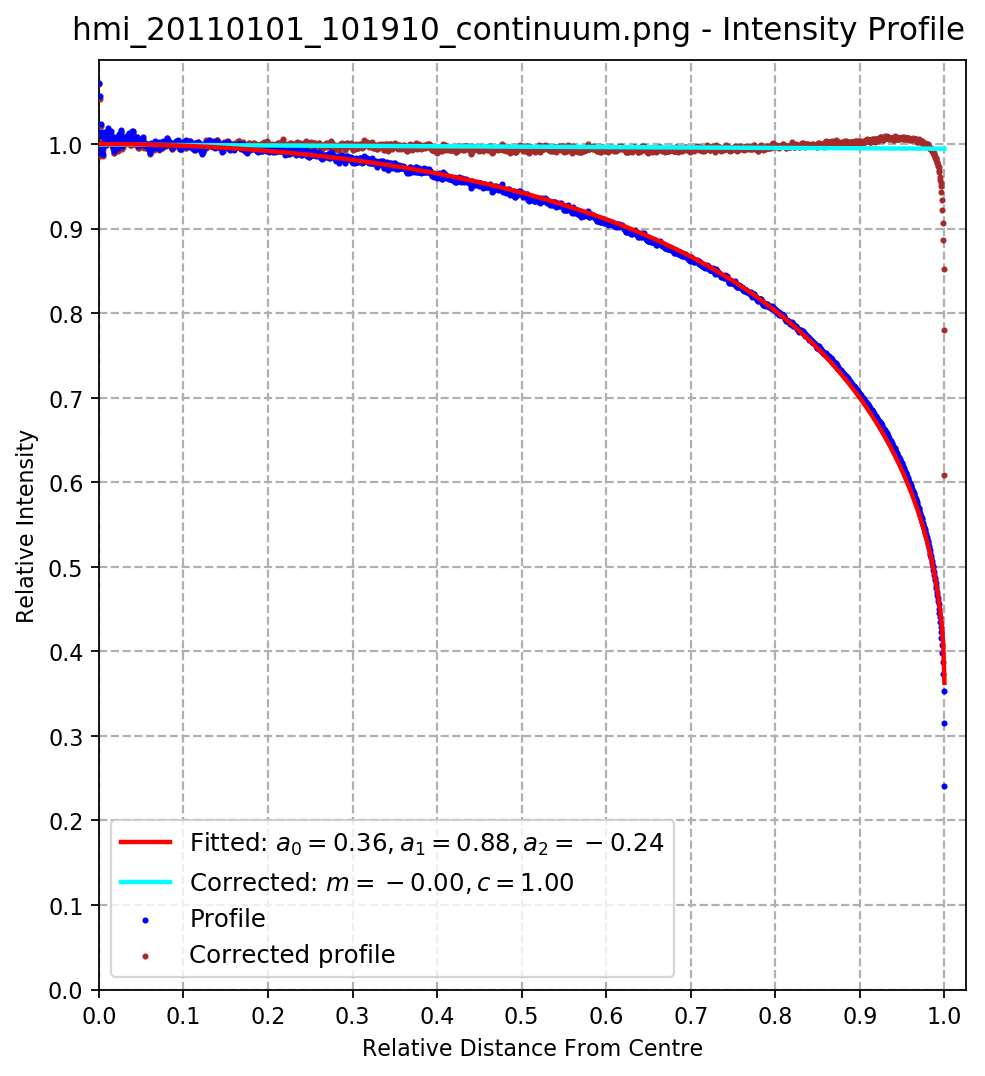
\includegraphics[width=\textwidth]{./pictures/SLDTk}
    \caption{Limb darkening intnsity profile created with SLDTk \cite{sldtk}.}
    \label{fig:sldtk}
\end{figure}\\
Once the coordinates of the sunspots are ready for both ground and space observations, the segmentation masks can be generated by a flooding procedure. For each sunspot a seed is initialized from its coordinates. From the seed, the procedure starts to explore the pixels around it in a breadth first fashion, so that for every iteration the pixels with lowest value are selected for expansion. By doing so, the algorithm floods the darkest areas of the image first, remaining trapped into the penumbra. Using the whole spot area provided by DPD, it is possible to calculte the exact number of pixels of each sunspot and therefore make the expansion stop exactly on the edge of the penumbra. All the pixels that have been selected at least once are then written on a black array that has the same shape of the original image, to create the segmentation mask. Actually, the final mask also contains information about the groups and their classes in order to train the second part of the algorithm. The annotations created by this procedure are consistently good in practice, as it can be appreciated from Figure~\ref{fig:annotated-sunspot}. The figure also shows how the precision of the mask increases with the size of sunspots. For instance, the contours of the small rightmost sunspots are not correctly captured in the mask, while the largest ones are almost perfectly represented.\\
\begin{figure}[t!]
    \centering
    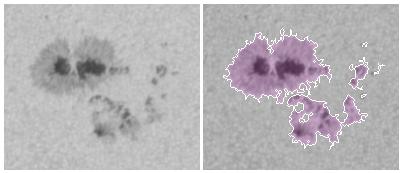
\includegraphics[width=\textwidth]{./pictures/blanquish}
    \caption{Example of a sunspot group mask.}
    \label{fig:annotated-sunspot}
\end{figure}
Overall, data preparation was probably the hardest and most time consuming part of the work, but the results repay the effort. The final analysis on the dataset shows the following statistics:
\begin{itemize}
  \item 2555 images with 4K resolution;
  \item around 21000 sunspot group instances;
  \item around 190000 single sunspots;
\end{itemize}
However, in order to train the algorithm and be able to asses its performance, it is necessary to divide the dataset into three subsets:
\begin{enumerate}
  \item \textbf{training set}: the part of data the algorithm will learn from;
  \item \textbf{validation set}: the sample of data that is used to provide an unbiased evaluation of the model while tuning hyperparameters. In our case the validation set will be particularly useful to estimate the personal reduction coefficient ($k$);
  \item \textbf{test set}: the chunk of data that will be used to estimate the final performance of the model once it is completely trained.
\end{enumerate}
The dataset was split accordingly trying to minimize the dependencies among the subsets. The initial idea was to split the dataset randomly, sampling observations for each month. This would have enabled us to estimate more precisely the average monthly sunspot number in the testing phase, because the observations would have been homogeneously distributed. Unfortunately, this is not a good approach because it introduces strong dependencies in the data, since sunspots can last even more than ten days on the disk and therefore the same sunspot could have appeared in both training and test data. A simple strategy is to divide the dataset while reducing regularities is to sample observations consecutively for the validation and test sets. So for each month the data was partitioned as follows:
\begin{itemize}
  \item days from the 1\textsuperscript{st} to the 19\textsuperscript{th} were assigned to the training set;
  \item days from the 20\textsuperscript{th} to the 24\textsuperscript{th} were assigned to the validation set;
  \item days from the 25\textsuperscript{th} to the last one of the month were assigned to the test set;
\end{itemize}
This data split design doesn't completely solve the dependency problem. In fact, though harder, it is still possible that the same sunspot appears repeated among the three sets. However, the longer the sunspot survives on the disk the more deformation it undergoes, strongly mitigating the dependency issue. Also, this partitioning strategy is a good trade-off because it still enables us to make monthly activity charts, averaging the results over the test set.
\clearpage
